\documentclass{beamer}

\usepackage{kotex}
\usepackage{graphicx,psfrag,amsfonts,amsmath,amssymb}
\usepackage{multicol}
\usepackage{algorithm2e}

\usetheme{metropolis}
\usefonttheme[onlymath]{serif}	% 수식 설정!!
\setbeamertemplate{section in toc}[sections numbered]

\title{Functional Classification for Sparse Data}
%\date{\today}
\date[Short Occasion]{September 9, 2019}
\author{Hyunsung Kim}
\institute{Department of Statistics\\ Chung-Ang University}

% A subtitle is optional and this may be deleted
\subtitle{}

%\author{F.~Author\inst{1} \and S.~Another\inst{2}}
% - Give the names in the same order as the appear in the paper.
% - Use the \inst{?} command only if the authors have different
%   affiliation.

%\institute[Universities of Somewhere and Elsewhere] % (optional, but mostly needed)
%{
%  \inst{1}%
%  Department of Computer Science\\
%  University of Somewhere
%  \and
%  \inst{2}%
%  Department of Theoretical Philosophy\\
%  University of Elsewhere}
% - Use the \inst command only if there are several affiliations.
% - Keep it simple, no one is interested in your street address.

%\date{Conference Name, 2013}
% - Either use conference name or its abbreviation.
% - Not really informative to the audience, more for people (including
%   yourself) who are reading the slides online

\subject{Functional Data Analysis}
% This is only inserted into the PDF information catalog. Can be left
% out. 

% If you have a file called "university-logo-filename.xxx", where xxx
% is a graphic format that can be processed by latex or pdflatex,
% resp., then you can add a logo as follows:

% \pgfdeclareimage[height=0.5cm]{university-logo}{university-logo-filename}
% \logo{\pgfuseimage{university-logo}}

% Delete this, if you do not want the table of contents to pop up at
% the beginning of each subsection:
\AtBeginSubsection[]
{
  \begin{frame}<beamer>{Outline}
    \tableofcontents[currentsection,currentsubsection]
  \end{frame}
}

\def \bY {\mathbf{Y}}
\def \by {\mathbf{y}}
\def \bX {\mathbf{X}}
\def \bB {\mathbf{B}}
\def \bD {\mathbf{D}}
\def \bbeta {\boldsymbol{\beta}}
\def \btheta {\boldsymbol{\theta}}
\def \bTheta {\boldsymbol{\Theta}}
\def \bepsilon {\boldsymbol{\epsilon}}
\def \balpha {\boldsymbol{\alpha}}
\def \bgamma {\boldsymbol{\gamma}}
\def \bGamma {\boldsymbol{\Gamma}}
\def \bR {\boldsymbol{R}}
\def \bZ {\boldsymbol{Z}}
\def \bG {\boldsymbol{G}}
\def \bu {\boldsymbol{u}}
\def \bV {\boldsymbol{V}}


% Let's get started
\begin{document}

\begin{frame}
  \titlepage
\end{frame}

\begin{frame}{Outline}
  \tableofcontents
  % You might wish to add the option [pausesections]
\end{frame}

% Section and subsections will appear in the presentation overview
% and table of contents.
\section{\texttt{fpca} package}
\begin{frame}{\texttt{fpca} package}
	\begin{block}{\texttt{fpca} package}
		\vspace{0.1cm}
		\begin{itemize}
			\item {
				The package to obtain functional PC for sparsely and irregularly observed data.
			}
			\item {
				Using the \texttt{EM} option, it solves the reduced rank model(James \textit{et al.}) to obtain FPC functions.
			}		
			\item {
				It uses PACE method(Yao \textit{et al.}) not the numerical integration to estimate FPC scores.
			}
		\end{itemize}
	\end{block}
\end{frame}

\begin{frame}{Comparison for Karhunen-Lo\`{e}ve Expansion}
	\begin{figure}[h] %%% t: top, b: bottom, h: here
		\begin{center}
			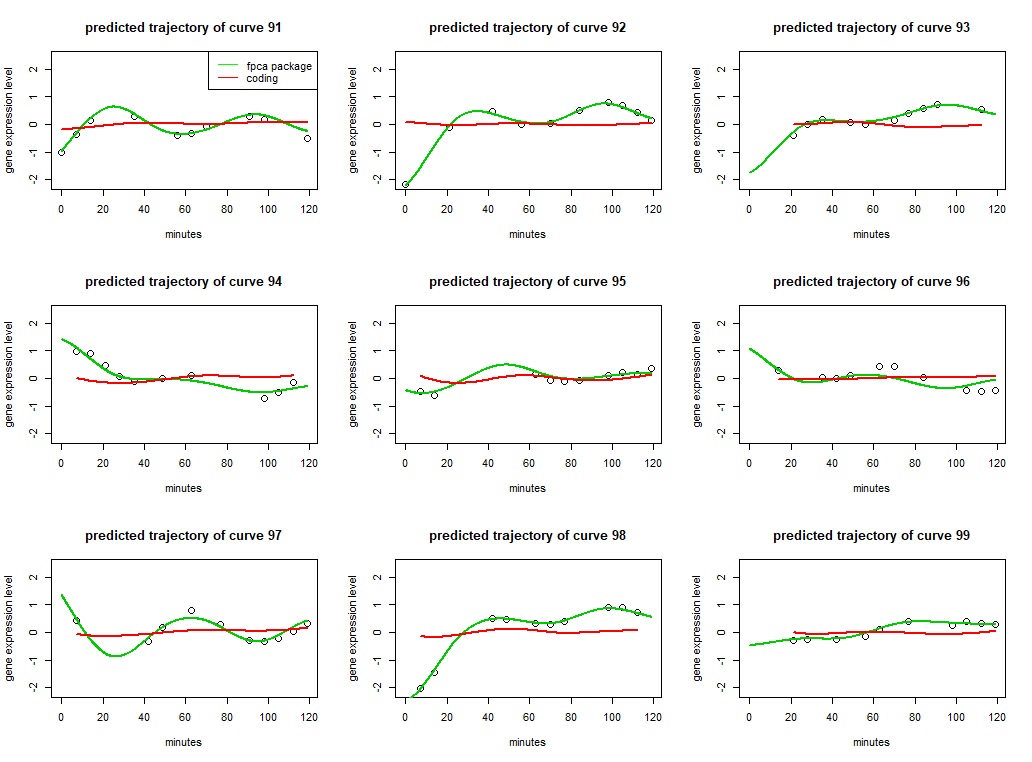
\includegraphics[width=0.8\linewidth]{img/1.png}
		\end{center}
		\label{fig:long}
		\label{fig:onecol}
		\caption{Predicted curves using 3 FPCs for 1st training set}
	\end{figure}
\end{frame}


\section{Simulation}
\begin{frame}{Simulation}
	\begin{block}{The Classification Methods}
		\vspace{0.1cm}
		\begin{itemize}
			\item {
				Functional logistic regression
			}
			\item {
				 SVM using FPCs with $4$ different kernels
			}
			\begin{itemize}
				\item {
					Linear
				}
				\item {
					Gaussian(Radial basis function)
				}
				\item {
					Sigmoid
				}
				\item {
					Polynomial
				}
			\end{itemize}
		\end{itemize}
	\end{block}
\end{frame}

\begin{frame}{Simulation}
	\begin{block}{The Procedure of the Simulation}
		\vspace{0.1cm}
		\begin{itemize}
			\item {
				Generate the $100$ datasets from the temporal gene expression data and 
				split the each dataset with training and test set.
			}
			\item {
				"Sparsify" the each dataset.
			}		
			\item {
				Estimate the FPC functions and scores using the sparse FPCA method with $7$ knots.
			}
			\item {
				Perform the $5$ classification methods for the training sets, and predict for the test sets with the different number of FPCs.
			}
%			\item {
%				The $100$ datasets are simulated from the first $5$ estimated FPCs from the temporal gene expression data.
%			}
%			\item {
%				 Each dataset has $200$ curves with 2 groups($G_1, G_2$)
%				 and is randomely divided to $100$ training and test sets for each.
%			}
%			\item {
%				We perform the functional logistic regression for the training sets, and predict for the test sets.
%			}
		\end{itemize}
	\end{block}
\end{frame}



\begin{frame}{Simulation Results}
	\begin{table}[ht]
		\caption{Accuracy using $2$ FPCs}
		\centering
		\tiny
		\begin{tabular}{cccccc}
			\hline
			No. of obs & Logistic & SVM(Linear) & SVM(Gaussian) & SVM(Sigmoid) & SVM(Polynomial) \\ 
			\hline
			2  & 0.560 & 0.553 & 0.551 & 0.554 & 0.530 \\ 
			3  & 0.685 & 0.684 & 0.652 & 0.669 & 0.643 \\ 
			4  & 0.743 & 0.743 & 0.729 & 0.719 & 0.709 \\ 
			5  & 0.777 & 0.775 & 0.757 & 0.762 & 0.735 \\ 
			6  & 0.788 & 0.787 & 0.770 & 0.771 & 0.747 \\ 
			7  & \textcolor{red}{0.793} & \textcolor{red}{0.791} & \textcolor{red}{0.779} & \textcolor{red}{0.779} & 0.754 \\ 
			8  & 0.789 & 0.786 & 0.771 & 0.767 & \textcolor{red}{0.755} \\ 
			9  & 0.784 & 0.783 & 0.767 & 0.767 & 0.745 \\ 
			10 & 0.784 & 0.782 & 0.769 & 0.772 & 0.751 \\ 
			11 & 0.775 & 0.775 & 0.761 & 0.759 & 0.744 \\ 
			12 & 0.789 & 0.787 & 0.770 & 0.775 & 0.759 \\ 
			13 & 0.781 & 0.783 & 0.768 & 0.762 & 0.752 \\ 
			14 & 0.784 & 0.784 & 0.769 & 0.770 & 0.752 \\ 
			15 & 0.779 & 0.778 & 0.768 & 0.764 & 0.747 \\ 
			16 & 0.783 & 0.783 & 0.768 & 0.771 & 0.748 \\ 
			17 & 0.779 & 0.780 & 0.764 & 0.757 & 0.746 \\ 
			18 & 0.781 & 0.778 & 0.764 & 0.766 & 0.748 \\ 
			\hline
			Average & 0.762 & 0.761 & 0.746 & 0.746 & 0.727 \\
			\hline
		\end{tabular}
	\end{table}
\end{frame}

\begin{frame}{Simulation Results}
	\begin{table}[ht]
		\caption{Accuracy using $3$ FPCs}
		\centering
		\tiny
		\begin{tabular}{cccccc}
			\hline
			No. of obs & Logistic & SVM(Linear) & SVM(Gaussian) & SVM(Sigmoid) & SVM(Polynomial) \\ 
			\hline
			2 & 0.549 & 0.547 & 0.551 & 0.533 & 0.556 \\ 
			3 & 0.750 & 0.742 & 0.712 & 0.731 & 0.707 \\ 
			4 & 0.801 & 0.804 & 0.790 & 0.789 & 0.783 \\ 
			5 & 0.852 & 0.849 & 0.831 & 0.844 & 0.825 \\ 
			6 & 0.861 & 0.862 & 0.845 & 0.854 & 0.842 \\ 
			7 & 0.885 & 0.885 & 0.865 & 0.876 & 0.860 \\ 
			8 & 0.879 & 0.881 & 0.867 & 0.874 & 0.862 \\ 
			9 & 0.887 & 0.888 & 0.872 & 0.876 & 0.860 \\ 
			10 & 0.894 & 0.894 & 0.878 & 0.885 & 0.876 \\ 
			11 & 0.881 & 0.886 & 0.868 & 0.877 & 0.859 \\ 
			12 & 0.892 & 0.893 & 0.874 & 0.883 & 0.872 \\ 
			13 & 0.893 & 0.891 & 0.879 & 0.885 & 0.869 \\ 
			14 & 0.894 & 0.897 & 0.881 & 0.888 & 0.875 \\ 
			15 & 0.893 & 0.896 & 0.882 & 0.887 & 0.874 \\ 
			16 & 0.896 & \textcolor{red}{0.899} & 0.884 & 0.885 & 0.877 \\ 
			17 & 0.896 & 0.898 & \textcolor{red}{0.885} & \textcolor{red}{0.889} & \textcolor{red}{0.878} \\ 
			18 & \textcolor{red}{0.897} & 0.898 & \textcolor{red}{0.885} & \textcolor{red}{0.889} & 0.877 \\ 
			\hline
			Average & 0.853 & 0.854 & 0.838 & 0.844 & 0.832 \\
			\hline
		\end{tabular}
	\end{table}
\end{frame}

\begin{frame}{Simulation Results}
	\begin{table}[ht]
		\caption{Accuracy using $4$ FPCs}
		\centering
		\tiny
		\begin{tabular}{cccccc}
			\hline
			No. of obs & Logistic & SVM(Linear) & SVM(Gaussian) & SVM(Sigmoid) & SVM(Polynomial) \\ 
			\hline
			2  & 0.554 & 0.568 & 0.552 & 0.566 & 0.598 \\ 
			3  & 0.699 & 0.711 & 0.678 & 0.690 & 0.656 \\ 
			4  & 0.812 & 0.811 & 0.771 & 0.796 & 0.769 \\ 
			5  & 0.863 & 0.860 & 0.834 & 0.847 & 0.821 \\ 
			6  & 0.876 & 0.874 & 0.856 & 0.863 & 0.845 \\ 
			7  & 0.883 & 0.885 & 0.859 & 0.874 & 0.855 \\ 
			8  & 0.886 & 0.890 & 0.861 & 0.881 & 0.860 \\ 
			9  & 0.897 & 0.900 & 0.876 & 0.886 & 0.875 \\ 
			10 & \textcolor{red}{0.903} & 0.902 & 0.875 & 0.893 & 0.871 \\ 
			11 & 0.896 & 0.897 & 0.879 & 0.889 & 0.872 \\ 
			12 & 0.898 & 0.900 & 0.877 & 0.887 & 0.874 \\ 
			13 & 0.895 & 0.899 & 0.879 & 0.888 & 0.872 \\ 
			14 & 0.902 & \textcolor{red}{0.905} & 0.880 & 0.890 & 0.875 \\ 
			15 & 0.900 & 0.902 & 0.881 & 0.891 & 0.875 \\ 
			16 & 0.901 & \textcolor{red}{0.905} & \textcolor{red}{0.885} & 0.894 & \textcolor{red}{0.879} \\ 
			17 & 0.900 & 0.904 & \textcolor{red}{0.885} & \textcolor{red}{0.897} & 0.878 \\ 
			18 & 0.902 & \textcolor{red}{0.905} & 0.883 & 0.892 & 0.877 \\ 
			\hline
			Average & 0.857 & 0.860 & 0.836 & 0.849 & 0.833 \\
			\hline
		\end{tabular}
	\end{table}
\end{frame}

\begin{frame}{Simulation Results}
	\begin{table}[ht]
		\caption{Accuracy using $5$ FPCs}
		\centering
		\tiny
		\begin{tabular}{cccccc}
			\hline
			No. of obs & Logistic & SVM(Linear) & SVM(Gaussian) & SVM(Sigmoid) & SVM(Polynomial) \\ 
			\hline
			2  & 0.518 & 0.537 & 0.523 & 0.537 & 0.502 \\ 
			3  & 0.623 & 0.632 & 0.622 & 0.603 & 0.596 \\ 
			4  & 0.678 & 0.680 & 0.641 & 0.661 & 0.645 \\ 
			5  & 0.854 & 0.855 & 0.815 & 0.843 & 0.823 \\ 
			6  & 0.865 & 0.866 & 0.834 & 0.851 & 0.835 \\ 
			7  & 0.894 & 0.896 & 0.868 & 0.882 & 0.866 \\ 
			8  & 0.889 & 0.889 & 0.866 & 0.882 & 0.865 \\ 
			9  & 0.898 & 0.895 & 0.867 & 0.887 & 0.873 \\ 
			10 & 0.897 & 0.896 & 0.869 & 0.890 & 0.872 \\ 
			11 & \textcolor{red}{0.900} & 0.901 & 0.872 & 0.891 & 0.877 \\ 
			12 & \textcolor{red}{0.900} & 0.901 & 0.876 & 0.889 & 0.874 \\ 
			13 & 0.896 & 0.899 & 0.876 & 0.891 & 0.873 \\ 
			14 & 0.898 & 0.902 & 0.877 & 0.890 & 0.875 \\ 
			15 & 0.899 & 0.903 & 0.874 & 0.890 & 0.876 \\ 
			16 & \textcolor{red}{0.900} & 0.904 & 0.877 & \textcolor{red}{0.894} & \textcolor{red}{0.879} \\ 
			17 & 0.898 & 0.902 & \textcolor{red}{0.878} & 0.892 & 0.877 \\ 
			18 & \textcolor{red}{0.900} & \textcolor{red}{0.905} & 0.875 & 0.889 & \textcolor{red}{0.879} \\ 
			\hline
			Average & 0.842 & 0.845 & 0.818 & 0.833 & 0.817 \\
			\hline
		\end{tabular}
	\end{table}
\end{frame}

\begin{frame}{Simulation Results}
	\begin{block}{Comparison between 5 Classification methods}
		\vspace{0.1cm}
		\begin{itemize}
			\item {
				The logistic regression and linear SVM perform well than other kernel SVM methods.
			}
			\item {
				When the number of FPCs is greater than or equal to $3$, the accuracy is very similar.
			}
			\item {
				If there are about $7$ out of $18$ observations, the accuracy is almost the same.
			}
		\end{itemize}
	\end{block}
\end{frame}


\appendix
\section{Reference}
\begin{frame}
  \frametitle<presentation>{Reference}
    
  \begin{thebibliography}{10}
  	\beamertemplatearticlebibitems
	% Followed by interesting articles. Keep the list short. 
	 \bibitem{Someone2000}
		%GARETH M. JAMES, TREVOR J. HASTIE, CATHERINE A. SUGAR
		James G.M. \textit{et al.}
		\newblock Principal component models for sparse functional data
		\newblock {\em Biometrika}, 87(3):587--602,
		2000.
		
   	\beamertemplatearticlebibitems
	\bibitem{Someone2005}
		Yao F. \textit{et al.}
		\newblock Functional data analysis for sparse longitudinal data
		\newblock {\em Journal of the American Statistical Association}, 100(470):577--590,
		2005.
	
   	\beamertemplatearticlebibitems
		\bibitem{Someone2006}
		 Rossi F. and Villa N. \textit{et al.}
		 \newblock Support vector machine for functional data classification
		 \newblock {\em Neurocomputing}, 69:730--742,
		 2006.
    
    \beamertemplatearticlebibitems
    \bibitem{Someone2006}
    Leng. X. and Müller. HG.
    \newblock Classification using functional data analysis for temporal gene expression data
    \newblock {\em Bioinformatics}, 22(1):68--76,
    2006.

  \end{thebibliography}
\end{frame}


% All of the following is optional and typically not needed. 
%\appendix
%\section<presentation>*{\appendixname}
%\subsection<presentation>*{For Further Reading}
%
%\begin{frame}[allowframebreaks]
%  \frametitle<presentation>{For Further Reading}
%    
%  \begin{thebibliography}{10}
%    
%  \beamertemplatebookbibitems
%  % Start with overview books.
%
%  \bibitem{Author1990}
%    A.~Author.
%    \newblock {\em Handbook of Everything}.
%    \newblock Some Press, 1990.
% 
%    
%  \beamertemplatearticlebibitems
%  % Followed by interesting articles. Keep the list short. 
%
%  \bibitem{Someone2000}
%    S.~Someone.
%    \newblock On this and that.
%    \newblock {\em Journal of This and That}, 2(1):50--100,
%    2000.
%  \end{thebibliography}
%\end{frame}

\end{document}


